% !TEX root = ../main.tex
% File: chapters_part1/chap3_2.tex
% Nội dung cho Phần 3.2: Autoencoders cho Biểu diễn Văn bản

\section{Autoencoders: Học Biểu diễn Phi giám sát}
\label{ssec:autoencoders}

Trong khi Word2Vec học biểu diễn cho từng từ riêng lẻ, một câu hỏi tự nhiên được đặt ra: Làm thế nào để chúng ta có thể học được một vector biểu diễn \textbf{cho cả một câu hoặc một tài liệu}? Một trong những câu trả lời kinh điển và mạnh mẽ nhất đến từ một kiến trúc mạng nơ-ron thanh lịch có tên là \textbf{Autoencoder (AE)}.

\subsection{Trực giác và Kiến trúc}

Ý tưởng cốt lõi của Autoencoder rất đơn giản nhưng vô cùng hiệu quả: Thay vì cố gắng dự đoán một nhãn bên ngoài, mô hình được giao một nhiệm vụ \textbf{tự giám sát} (self-supervised): \textit{hãy học cách tái tạo lại chính xác những gì nó nhìn thấy}.

Để làm được điều này một cách có ý nghĩa, kiến trúc của Autoencoder được thiết kế có chủ đích theo dạng "đồng hồ cát" (hourglass) gồm hai phần đối xứng:

\begin{itemize}
    \item \textbf{Bộ mã hóa (Encoder):} Phần đầu vào của "đồng hồ cát", có nhiệm vụ nhận một vector đầu vào $\mathbf{x}$ có số chiều lớn (ví dụ, một vector Bag-of-Words cho một câu) và \textbf{nén} nó xuống một vector biểu diễn ẩn $\mathbf{z}$ có số chiều nhỏ hơn nhiều. Vector $\mathbf{z}$ này được gọi là \textbf{biểu diễn tiềm ẩn} (latent representation) hoặc \textit{code}.
    \item \textbf{Bộ giải mã (Decoder):} Phần đầu ra của "đồng hồ cát", nhận vector nén $\mathbf{z}$ và cố gắng \textbf{giải nén} nó để tái tạo lại vector đầu vào ban đầu, ký hiệu là $\hat{\mathbf{x}}$.
\end{itemize}

\paragraph{Huấn luyện}
Mục tiêu của mạng là tối thiểu hóa \textbf{lỗi tái tạo (reconstruction error)}, tức là làm cho vector đầu ra $\hat{\mathbf{x}}$ càng giống vector đầu vào $\mathbf{x}$ càng tốt. Điều này được thực hiện bằng cách định nghĩa một \textbf{hàm mất mát}, ví dụ như sai số bình phương trung bình (Mean Squared Error - MSE):
$$ \mathcal{L}(\mathbf{x}, \hat{\mathbf{x}}) = \|\mathbf{x} - \hat{\mathbf{x}}\|^2 $$
Trong quá trình huấn luyện, lỗi này được lan truyền ngược (\textbf{backpropagation}) từ đầu ra trở về đầu vào, cập nhật các trọng số của cả Decoder và Encoder để chúng có thể tạo ra một biểu diễn nén $\mathbf{z}$ tốt hơn và tái tạo lại $\mathbf{x}$ chính xác hơn.

\begin{center}
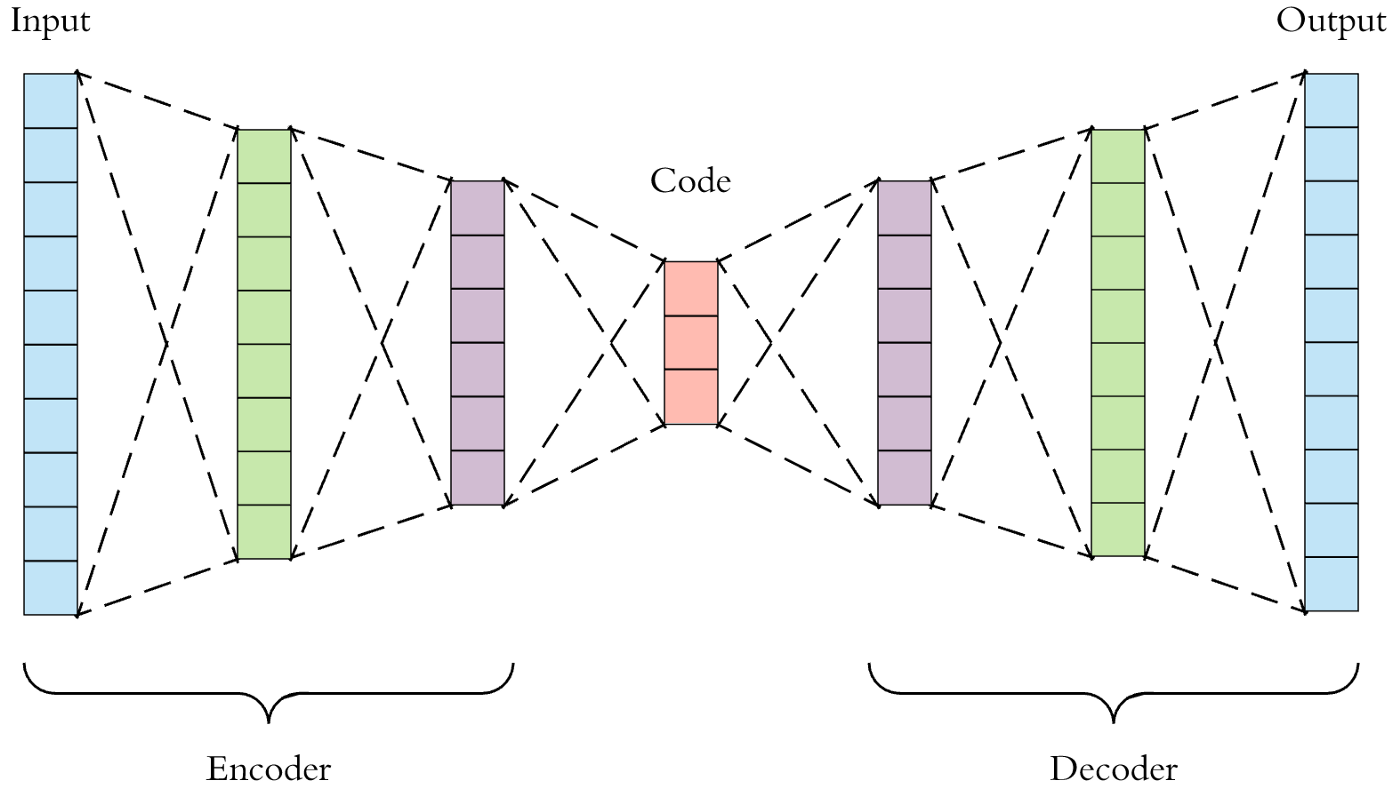
\includegraphics[width=0.7\textwidth]{autoencoder_structure.png}
\captionof{figure}{Kiến trúc tổng quát của Autoencoder. Phần hẹp nhất (\textit{bottleneck}) chính là không gian ẩn chứa thông tin nén.}
\label{fig:autoencoder_structure}
\end{center}

\subsection{Sức mạnh của "Nút cổ chai" và việc học biểu diễn}
Điểm mấu chốt làm cho Autoencoder trở nên hữu ích chính là lớp ẩn ở giữa có số chiều nhỏ, hay còn gọi là \textbf{"nút cổ chai" (bottleneck)}. Lớp này buộc mạng phải học một dạng nén dữ liệu thông minh.

Nếu không có nút cổ chai (tức là số chiều của $\mathbf{z}$ bằng hoặc lớn hơn số chiều của $\mathbf{x}$), mạng sẽ rất dễ dàng học được một \textbf{ánh xạ đồng nhất} (identity function) tầm thường. Nó chỉ đơn giản là sao chép đầu vào ra đầu ra mà không cần phải "hiểu" bất kỳ cấu trúc tiềm ẩn nào của dữ liệu. Một mô hình như vậy sẽ tái tạo đầu vào một cách hoàn hảo nhưng biểu diễn ẩn $\mathbf{z}$ sẽ không có giá trị tổng quát hóa.

Ngược lại, sự tồn tại của nút cổ chai đặt ra một thách thức: làm thế nào để đi qua một không gian hẹp như vậy mà vẫn giữ đủ thông tin để tái tạo lại đầu ra một cách chính xác? Điều này buộc bộ mã hóa phải học cách:
\begin{itemize}
    \item \textbf{Chắt lọc thông tin tinh túy:} Giữ lại những đặc trưng quan trọng nhất, có tính phân biệt cao nhất của dữ liệu.
    \item \textbf{Loại bỏ thông tin dư thừa và nhiễu:} Những chi tiết không cần thiết hoặc ngẫu nhiên sẽ bị loại bỏ trong quá trình nén.
    \item \textbf{Khai thác các mối tương quan:} Mô hình phải học được các quy luật và sự phụ thuộc lẫn nhau giữa các chiều của dữ liệu đầu vào để có thể nén chúng một cách hiệu quả.
\end{itemize}

\begin{displayquote}
    \textit{Mục tiêu thực sự của Autoencoder không phải là tái tạo đầu ra, mà là học được một \textbf{biểu diễn nén} ($\mathbf{z}$) giàu thông tin trong quá trình đó.}
\end{displayquote}

Sau khi huấn luyện xong, chúng ta thường sẽ loại bỏ phần Decoder và chỉ sử dụng phần Encoder như một công cụ trích xuất đặc trưng mạnh mẽ: đưa một câu vào và nhận về một vector biểu diễn dày đặc, giàu ngữ nghĩa.

\subsection{Ứng dụng và Các biến thể trong NLP}
\begin{tcolorbox}[
    title=Lựa chọn Thiết kế cho Autoencoder trong NLP,
    colback=orange!5!white, colframe=orange!60!black, fonttitle=\bfseries
]
Việc áp dụng Autoencoder cho văn bản đòi hỏi một số lựa chọn thiết kế quan trọng:
\begin{itemize}
    \item \textbf{Biểu diễn Đầu vào ($\mathbf{x}$):}
    \begin{itemize}
        \item \textbf{Bag-of-Words (BoW):} Đơn giản và phổ biến. Mô hình sẽ học cách tái tạo lại tần suất của các từ trong câu. Biểu diễn tiềm ẩn $\mathbf{z}$ khi đó có xu hướng nắm bắt các \textbf{chủ đề} (topics) chính của văn bản, vì đó là thông tin quan trọng nhất để tái tạo lại túi từ.
        \item \textbf{TF-IDF:} Tương tự BoW nhưng đã có trọng số cho các từ quan trọng. Điều này có thể giúp mô hình tập trung hơn vào các từ khóa có ý nghĩa.
        \item \textbf{Lưu ý:} Cả hai phương pháp trên đều làm mất thông tin về trật tự từ.
    \end{itemize}
    \item \textbf{Hàm mất mát (Reconstruction Error):}
    \begin{itemize}
        \item \textbf{Mean Squared Error (MSE):} Phù hợp với đầu vào có giá trị thực như TF-IDF. Tuy nhiên, với BoW (giá trị đếm), nó có thể không phải là lựa chọn lý tưởng nhất về mặt lý thuyết xác suất.
        \item \textbf{Cross-Entropy:} Một lựa chọn tốt hơn khi xem vector BoW (đã được chuẩn hóa) như một phân phối xác suất đa thức trên từ vựng. Hàm mất mát này sẽ cố gắng làm cho phân phối xác suất tái tạo $\hat{\mathbf{x}}$ gần với phân phối gốc $\mathbf{x}$ nhất có thể, thường cho kết quả tốt hơn trong thực tế.
    \end{itemize}
\end{itemize}
Sự kết hợp giữa biểu diễn đầu vào và hàm mất mát sẽ định hình những gì mà biểu diễn tiềm ẩn $\mathbf{z}$ học được. Ví dụ, với BoW và Cross-Entropy, $\mathbf{z}$ sẽ là một "bản tóm tắt chủ đề" hiệu quả của văn bản.
\end{tcolorbox}
Trong NLP, Autoencoder và các biến thể của nó mở ra nhiều ứng dụng quan trọng:
\begin{itemize}
    \item \textbf{Học biểu diễn cho Câu/Đoạn văn:} Đây là ứng dụng cơ bản nhất, tạo ra các "sentence embeddings" chất lượng cao từ dữ liệu không gán nhãn, có thể được dùng cho các tác vụ phân cụm, tìm kiếm ngữ nghĩa, hoặc làm đặc trưng đầu vào cho các mô hình có giám sát.
    \item \textbf{Khởi tạo Trọng số (Pre-training):} Trước kỷ nguyên Transformer, các Autoencoder xếp chồng (Stacked Autoencoders) được dùng để khởi tạo trọng số cho từng lớp của một mạng nơ-ron sâu. Việc này giúp quá trình huấn luyện hội tụ nhanh hơn và tốt hơn.
    \item \textbf{Sinh Văn bản (Text Generation):} Mặc dù Autoencoder cơ bản là mô hình phân biệt, các biến thể của nó là nền tảng cho các mô hình sinh.
\end{itemize}

Một số biến thể phổ biến và có sức ảnh hưởng lớn bao gồm:

\begin{itemize}
    \item \textbf{Denoising Autoencoder (DAE) \cite{vincent2008extracting}:} Một ý tưởng đơn giản nhưng cực kỳ mạnh mẽ. Thay vì học cách tái tạo lại đầu vào $\mathbf{x}$, DAE được huấn luyện để tái tạo $\mathbf{x}$ từ một phiên bản đã bị làm hỏng (corrupted) của nó, $\tilde{\mathbf{x}}$ (ví dụ: một vài từ bị xóa hoặc thay thế ngẫu nhiên). Điều này buộc mô hình học được các biểu diễn \textbf{bền vững (robust)} hơn, không chỉ là nén mà còn phải "hiểu" để có thể "sửa lỗi".
    \item \textbf{Variational Autoencoder (VAE) \cite{kingma2013auto}:} Một bước nhảy vọt về mặt lý thuyết, biến Autoencoder thành một mô hình \textbf{sinh (generative model)} thực thụ. Thay vì mã hóa đầu vào thành một vector điểm $\mathbf{z}$ duy nhất, VAE mã hóa nó thành một \textbf{phân phối xác suất} (thường là phân phối Gaussian) trong không gian tiềm ẩn. Sau khi huấn luyện, chúng ta có thể lấy mẫu một vector $\mathbf{z}$ ngẫu nhiên từ phân phối này và đưa qua Decoder để sinh ra một mẫu dữ liệu mới hoàn toàn nhưng vẫn tương tự dữ liệu huấn luyện. Chúng ta sẽ thảo luận kỹ hơn về VAE trong Mục \ref{ssec:vae_for_text}.
    \item \textbf{Sequence-to-Sequence Autoencoder:} Thay vì dùng các lớp kết nối đầy đủ (fully-connected) cho văn bản dạng Bag-of-Words, biến thể này sử dụng các kiến trúc tuần tự như \textbf{RNN/LSTM} cho cả Encoder và Decoder. Encoder đọc một chuỗi từ và nén nó thành một vector "tư tưởng" (thought vector), sau đó Decoder sẽ cố gắng tái tạo lại chính chuỗi từ đó từ vector này. Đây chính là tiền đề cho kiến trúc Encoder-Decoder trong các bài toán Seq2Seq như dịch máy.
\end{itemize}

Tóm lại, Autoencoder là một công cụ học phi giám sát nền tảng, cung cấp một phương pháp hiệu quả để học các biểu diễn nén, giàu ngữ nghĩa cho các đơn vị văn bản lớn hơn từ. Ý tưởng về việc học thông qua tái tạo và nén qua "nút cổ chai" là một trong những khái niệm có sức ảnh hưởng sâu rộng trong học sâu hiện đại.